\documentclass[11pt,openany]{book}
\raggedbottom

% ===================================================================
%                          Package Loading
% ===================================================================
\usepackage[utf8]{inputenc} % for unicode input
\usepackage{microtype}
\usepackage{bm}
\usepackage{enumitem}
\usepackage{geometry} % for page layout
\usepackage{hyperref} % for hyperlinks
\usepackage{tocbibind} % includes the bibliography in the table of contents
\usepackage{amsmath, amsfonts, amssymb, amsthm} % for advanced math formatting
\usepackage{lipsum} % generates filler text
\usepackage{fancyhdr}
\usepackage[table]{xcolor} % for cell coloring
\usepackage{graphicx} % for including images
\usepackage{booktabs} % for professional looking tables
\usepackage[normalem]{ulem} % for underlining
\usepackage[document]{ragged2e} % for text alignment
\usepackage{tikz} % for drawing
\usepackage{algorithm}
\usepackage{algpseudocode}
\usepackage{wrapfig}
\usepackage{circuitikz}
\usepackage{caption}
\usepackage{venndiagram}
\usepackage{multicol}
\usepackage{listings}
\usepackage{adjustbox}
\usepackage{multirow}
\newcommand{\dist}[2]{\left\langle #1,\, #2 \right\rangle}

%\usepackage{amsthm}
\usepackage{tcolorbox}
\tcbuselibrary{theorems,skins,breakable}
\usepackage{tikz}
\usepackage{xcolor}




% Link counters with amsthm
\newtheorem{definition}{Definition}[section]
\newtheorem{theorem}{Theorem}[section]
\newtheorem{example}{Example}[section]


% Document geometry (page size, margins)
\geometry{a4paper, left=20mm, right=20mm, top=25mm, bottom=30mm}

% Set header height for fancyhdr
\setlength{\headheight}{14pt}

% Custom page style for centered page numbers
\pagestyle{fancy}
\fancyhf{} % Clear all header and footer fields
\fancyhead[RE]{\leftmark} % Left Even pages - Chapter number and name
\fancyhead[RO]{Notes by Ali EL AZDI} % Right Odd pages - Custom message
\fancyfoot[CE,CO]{\thepage} % Centered page number in the footer
\renewcommand{\headrulewidth}{0pt}
\renewcommand{\footrulewidth}{0pt}


% ===================================================================
%                        Document Begins
% ===================================================================
\begin{document}

% -------------------------------------------------------------------
%                            Title Page
% -------------------------------------------------------------------
\begin{titlepage}
    \centering
    \vspace*{1cm}
    {\Huge Analysis III - Distribution Theory} \\
    \vspace{10px}
    {\LARGE IN~BA3 - Martin Werner Licht} \\
    \vspace*{1cm}
    {\Large Notes by Ali EL AZDI} \\
    \vfill
    {\large November 6, 2024}
\end{titlepage}

% -------------------------------------------------------------------
%                        Introduction Note
% -------------------------------------------------------------------
\begin{center}
    \vspace*{1cm}
    \textbf{Introduction}

    \paragraph[short]{}{\justifying This document is designed to provide a concise, step-by-step introduction to \textit{Distribution Theory}, often referred to as the theory of generalized functions. The notes follow a clean and clear exposition style, illustrating concepts with simple examples. Should you discover any inaccuracies or have suggestions for improvements, please reach out at \texttt{ali.elazdi@epfl.ch}. Alternatively, you can contribute via a pull request if you wish to propose significant changes, additions, or corrections to the course content.}
\end{center}

% -------------------------------------------------------------------
%                        Table of Contents
% -------------------------------------------------------------------
\tableofcontents

% ===================================================================
%                  Chapter 1: Distribution Theory
% ===================================================================
\chapter{Introduction to Distribution Theory}

% -------------------------------------------------------------------
%                        Overview
% -------------------------------------------------------------------
\noindent
\textit{This course aims to establish a rigorous framework for generalized functions, show why objects like the Dirac Delta require a broader viewpoint than classical functions, and equip readers with the essential tools to work with these distributions.}

\vskip 1em

\section{Course I - Introduction to Distribution Theory}
\noindent
\textbf{Motivation.}
In classical analysis, certain “functions” (like the Dirac Delta) don't exist in the usual sense but arise naturally in differential equations and signal processing. Instead of evaluating pointwise, we probe functions by integrating them against well-chosen, smooth “test” functions, capturing broader features rather than individual values.


% -------------------------------------------------------------------
%             Subsection: Probing Functions via Integration
% -------------------------------------------------------------------
\subsection{Probing Functions via Integration}

One of the core ideas in Distribution Theory is the concept of \textit{testing} or \textit{probing} a function by integrating it against another. Rather than focusing on pointwise values, we explore how a given function behaves when combined with various smooth functions under the integral sign. \\ \smallskip
\noindent \textbf{Key Idea:} If \(\varphi : \mathbb{R} \to \mathbb{R}\) and \(g : \mathbb{R} \to \mathbb{R}\) are sufficiently nice functions (e.g., continuous, smooth, etc.), then we can explore:
    \[
    \int_{\mathbb{R}} \varphi(x)\, g(x)\, dx.
    \]
    This measures how \(\varphi\) and \(g\) \textit{interact} or \textit{overlap}.\\

\textit{By viewing functions through the lens of integrals against “test functions,” one can capture broad, “averaged” information about a function’s shape or behavior, rather than relying on individual point values.}
% -------------------------------------------------------------------
%                  Subsection: The Gaussian Bump
% -------------------------------------------------------------------
\newpage
\begin{example}[Gaussian Approximation.]
    \noindent \newline For \(\varepsilon > 0\), let's define
        \[
        g_\varepsilon(x) = \frac{1}{\sqrt{2\pi}\,\varepsilon}\, e^{-\frac{x^2}{\varepsilon^2}}.
        \]
        Each \(g_\varepsilon\) integrates to 1, and as \(\varepsilon \to 0\), it becomes sharply peaked at \(x = 0\). Hence, for a continuous function \(\varphi\),
        \[
        \lim_{\varepsilon \to 0}\int_{\mathbb{R}} \varphi(x)\,g_\varepsilon(x)\,dx = \varphi(0),
        \]
        mimicking evaluation at a point but through integrals. Although no ordinary function does this exactly, this limiting behavior paves the way to defining the Dirac Delta as a \emph{functional}.
    \end{example}
\begin{center}
    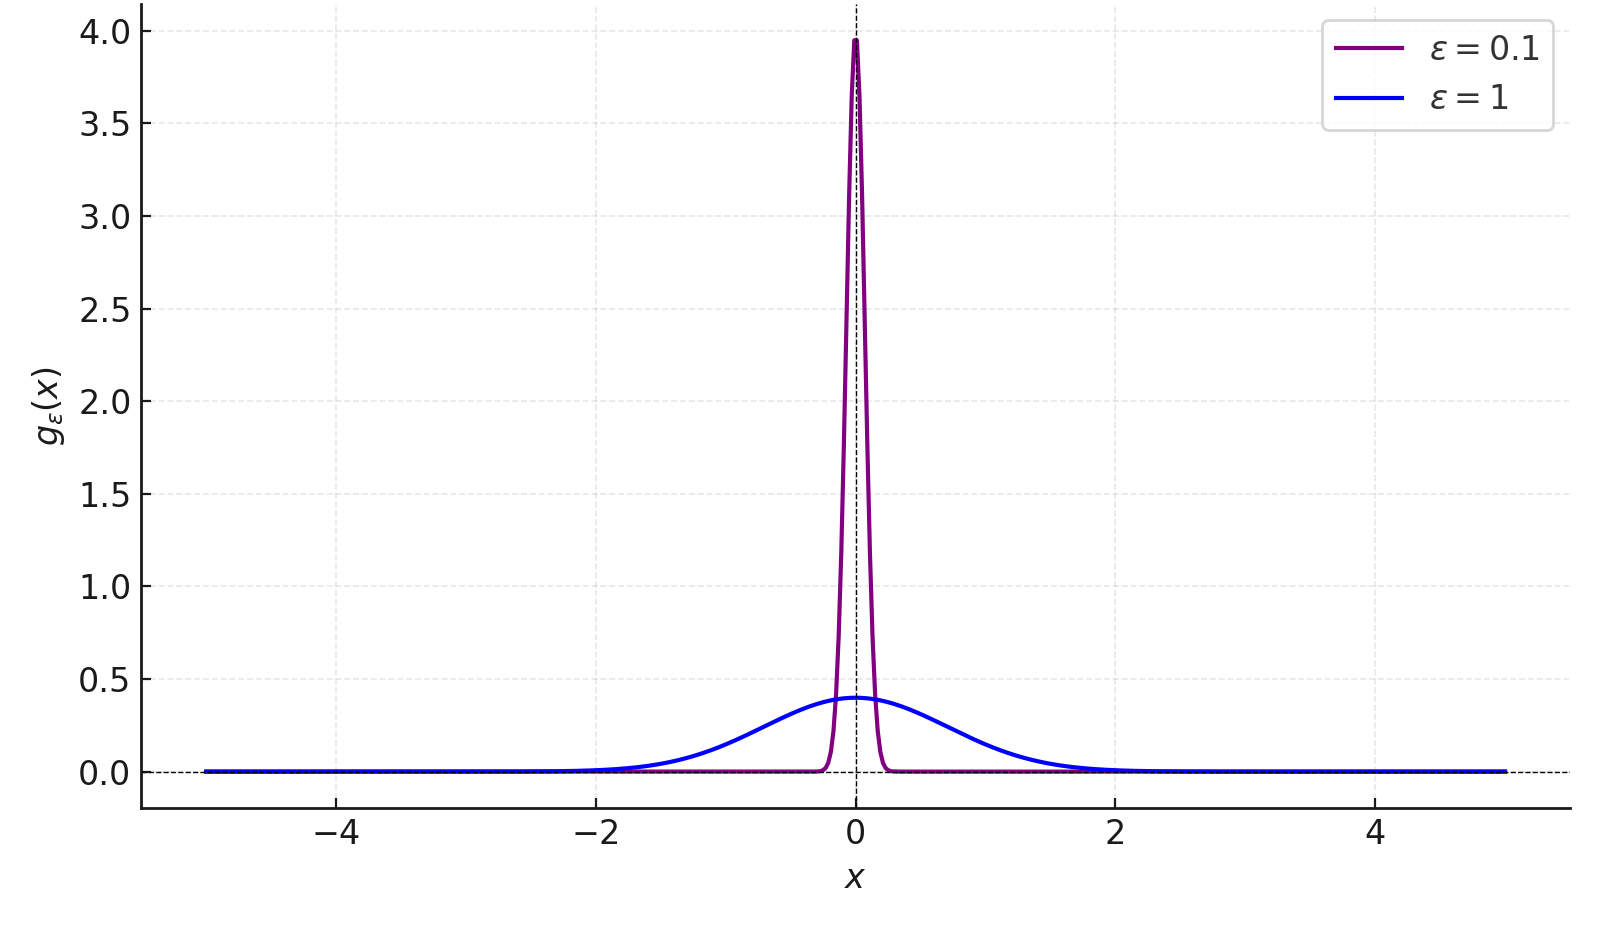
\includegraphics[width=0.65\textwidth]{images/gaussian_bump_plot.png}
\end{center}
\subsubsection{Normalization of \(g_\varepsilon\)}
Let's verify that \(g_\varepsilon\) integrates to one for each \(\varepsilon\). Consider:
\[
\int_{\mathbb{R}} g_\varepsilon(x)\, dx
= \frac{1}{\sqrt{2\pi}\,\varepsilon}
  \int_{\mathbb{R}} \exp\!\Bigl(-\frac{x^2}{\varepsilon^2}\Bigr)\, dx.
\]
By the substitution \(u = x / \varepsilon\), hence \(dx = \varepsilon\,du\), we obtain
\[
\int_{\mathbb{R}} \exp\!\Bigl(-\frac{x^2}{\varepsilon^2}\Bigr)\, dx
= \varepsilon \int_{\mathbb{R}} e^{-u^2}\, du
= \varepsilon \sqrt{\pi}.
\]
Thus,
\[
\int_{\mathbb{R}} g_\varepsilon(x)\, dx
= \frac{1}{\sqrt{2\pi}\,\varepsilon}\,\bigl(\varepsilon\sqrt{\pi}\bigr)
= 1.
\]

\noindent \textbf{Interpretation} \\
Because for each $\varepsilon$, \(g_\varepsilon\) has unit integral, the quantity
\[
\int_{\mathbb{R}} \varphi(x)\, g_\varepsilon(x)\, dx
\]
can be viewed as a weighted average of \(\varphi\), where the weights are dictated by the Gaussian shape \(g_\varepsilon\). As \(\varepsilon \to 0\), this integral concentrates around \(x=0\) and tends to evaluate \(\varphi\) at \(0\), at least for continuous \(\varphi\):
\[
\lim_{\varepsilon \to 0} \int_{\mathbb{R}} \varphi(x)\, g_\varepsilon(x)\, dx
= \varphi(0).
\]

% -------------------------------------------------------------------
%         Subsection: The Dirac Delta and Generalized Functions
% -------------------------------------------------------------------
\subsection{The Dirac Delta and Generalized Functions}

A major motivation for Distribution Theory is to rigorously handle the \textit{Dirac Delta}, denoted \(\delta_0\), which captures the idea of “point evaluation at zero” in an integral.

\subsubsection{Heuristic Motivation}

We might ask if there is a classical function \(g_0(x)\) such that
\[
\int_{\mathbb{R}} g_0(x)\,\varphi(x)\,dx = \varphi(0)
\quad
\text{for all test functions } \varphi(x).
\]
No ordinary function satisfies this. However, from the limiting behavior of the Gaussian family \(g_\varepsilon\), we see a suggestion that in some generalized sense, one can define:
\[
\delta_0[f] := f(0),
\]
meaning \(\delta_0\) is a \textit{functional} that takes a function \(f\) and returns its value at \(0\).

\subsubsection{A Functional, Not a Function}

The Dirac Delta is more properly viewed as a \textit{linear functional}:
\[
\delta_0 : C^0(\mathbb{R}) \,\to\, \mathbb{R},
\quad
f \,\mapsto\, f(0).
\]
It is not a genuine function in the classical sense but acts on functions by returning the value at a specific point.

\textbf{Heuristic Notation:} Physicists and engineers often write
\[
\int_{\mathbb{R}} \delta_0(x)\,f(x)\,dx = f(0),
\]
but strictly speaking, \(\delta_0\) is not a function. The equality holds in the distributional (generalized function) sense.
\newpage
% -------------------------------------------------------------------
%                      Section: Definitions
% -------------------------------------------------------------------
\section{Foundational Definitions}

To fully formalize these ideas, we need precise definitions of the underlying spaces of test functions and the generalized functions (distributions) themselves. Before diving into those spaces, we first clarify the notion of a function’s \textit{support}.

% -------------------------------------------------------------------
%         Subsection: Support of a Function - Definition
% -------------------------------------------------------------------
\subsection{Support of a Function}

\begin{definition}[Support]
For a function \(f: \mathbb{R} \to \mathbb{R}\), its \emph{support} is defined as the closure of the set where \(f\) is nonzero:
\[
\mathrm{supp}(f)
= \overline{\{\, x \in \mathbb{R} \mid f(x) \neq 0 \}}.
\]
\end{definition}

\begin{example} \noindent
For example \\
\smallskip
\begin{minipage}[t]{0.45\textwidth}
    $supp(f) = [a, b]$
    \centering
    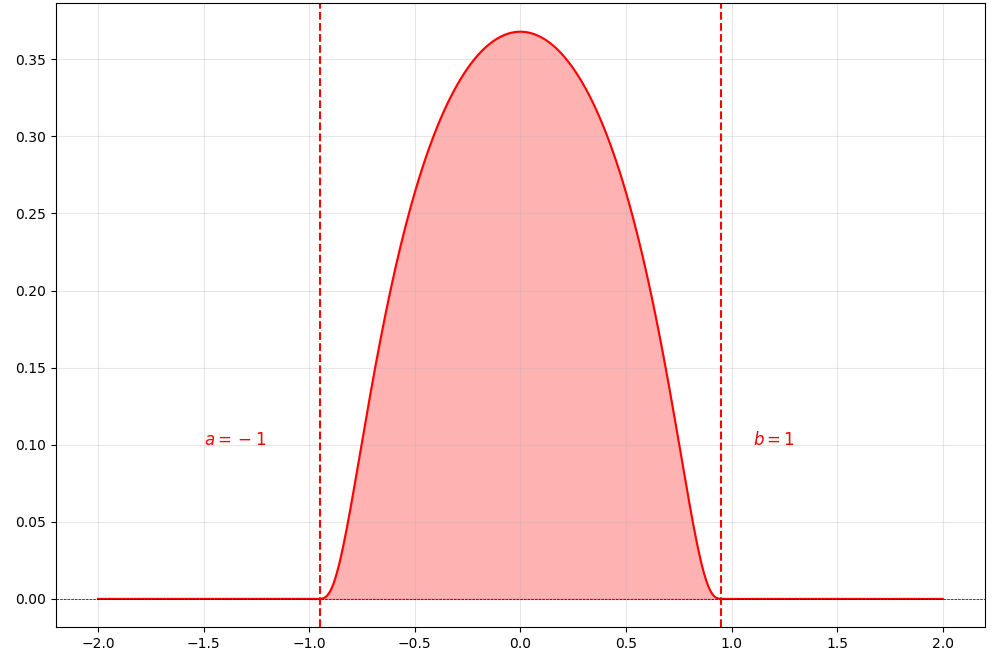
\includegraphics[width=0.95\textwidth]{images/support_single_interval.png}
\end{minipage}
\hfill
\vline
\hfill
\begin{minipage}[t]{0.45\textwidth}
    $supp(f) = [a, b] \cup [c, d]$
    \centering
    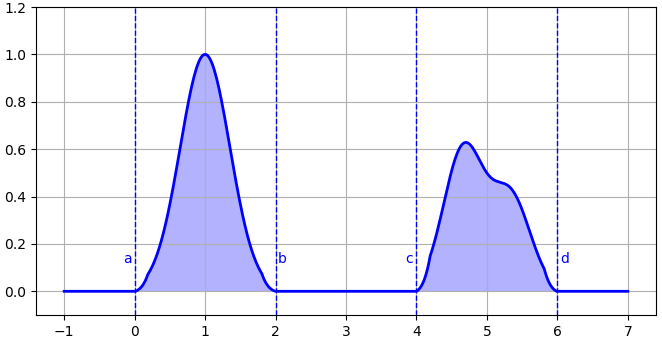
\includegraphics[width=1.20\textwidth]{images/support_union_intervals.png}
\end{minipage}
\end{example}



\noindent
If a function \(f\) is nonzero only in a finite union of intervals, its support is then precisely that union of intervals (closed). If \(f\equiv 0\) everywhere outside a certain bounded set, we say \(f\) has \textit{compact support}.

% -------------------------------------------------------------------
%          Subsection: Example - A Smooth Bump Function
% -------------------------------------------------------------------

\subsubsection*{A Closer Look at the Bump Function and Its Derivatives}

The function

\begin{minipage}[htp]{0.45\textwidth}
    \Large
    \[
\varphi(x) =
\begin{cases}
e^{-\frac{1}{\,1 - x^2\,}}, & |x| < 1,\\
0, & |x| \ge 1,
\end{cases}
\]
\normalsize
\end{minipage}
\hfill
\begin{minipage}[htp]{0.55\textwidth}
    \begin{center}
        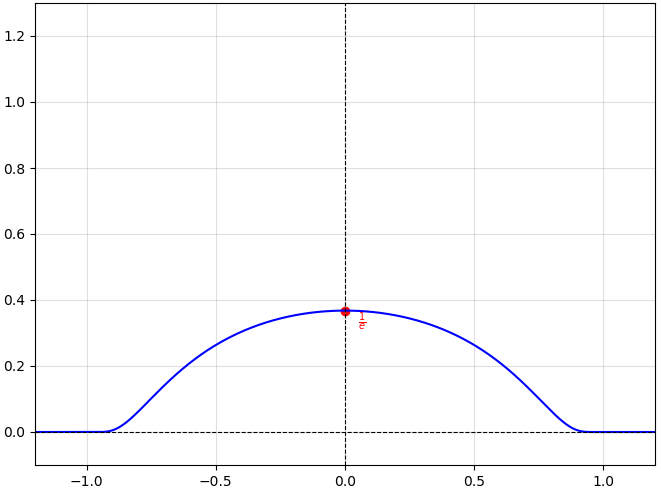
\includegraphics[width=0.9\textwidth]{images/phi.png}
    \end{center}
\end{minipage}\\
is smooth and compactly supported in $[-1,1]$. Despite looking piecewise, it belongs to $C^\infty(\mathbb{R})$ because both $\varphi$ and all its derivatives vanish seamlessly at $\pm 1$. Let us confirm this by examining its derivative.

\paragraph{Derivative Computation.}
For $|x| < 1$, using the chain rule, we compute:
\[
\varphi'(x)
= \frac{d}{dx} \bigl(e^{-\tfrac{1}{1 - x^2}}\bigr)
= e^{-\tfrac{1}{\,1 - x^2\,}}
   \;\times\;
   \bigl(-1\bigr)
   \;\times\;
   \frac{d}{dx}\bigl[\tfrac{1}{\,1 - x^2\,}\bigr].
\]
Since
\[
\frac{d}{dx}\Bigl[\tfrac{1}{\,1 - x^2\,}\Bigr]
= \frac{d}{dx}(1 - x^2)^{-1}
= -\, (1 - x^2)^{-2} \,\times\; \bigl(-2x\bigr)
= \frac{2x}{(1 - x^2)^2},
\]
we get
\[
\varphi'(x)
= e^{-\tfrac{1}{1 - x^2}}
  \times
  \frac{2x}{(1 - x^2)^2},
\]
for $|x|<1$, and $\varphi'(x)=0$ for $|x|\ge1$. \\
\medskip
\textbf{Behavior Near $x = \pm 1$.} \\
\noindent  Although the factor $\dfrac{2x}{(1 - x^2)^2}$ blows up as $x\to\pm 1$, the exponential term
$
e^{-\tfrac{1}{1 - x^2}}
$
goes to zero \emph{faster} than any power of $(1 - x^2)$ goes to infinity. Specifically, as $x \to \pm 1$, we have
$
-\frac{1}{1 - x^2}\;\to\; -\infty,
$
making $e^{-\frac{1}{1 - x^2}}\to 0$. Hence the product remains finite and actually tends to $0$ at $x=\pm 1$, guaranteeing continuity of $\varphi'$ at those boundary points. Repeated differentiation yields higher-order derivatives that similarly vanish outside $(-1,1)$ and remain smooth inside $(-1,1)$, so indeed $\varphi\in C^\infty_c(\mathbb{R})$.

\medskip
\begin{center}
  \hrulefill
\end{center}

\section{Preliminaries on Test Functions and Distributions}
\label{sec:testfunctions_distributions}

Distributions generalize the idea of functions by allowing us to make sense of certain \emph{function-like} objects (such as the Dirac Delta) that are not strictly definable as ordinary functions.

\subsection{The Space of Test Functions \texorpdfstring{$\mathcal{D}$}{D}}

\noindent
In Distribution Theory, we work with a special space of ``test'' functions:
\[
\mathcal{D} \;:=\; C_c^\infty(\mathbb{R})
\;=\;
\left\{\,
\psi \colon \mathbb{R}\to\mathbb{R}
 \;\middle|\;
 \psi \text{ is smooth and } \mathrm{supp}(\psi)\text{ is a bounded set}
\right\}.
\]
Any function $\psi \in \mathcal{D}$ is called a \emph{test function}.  We have just seen a prototype $\varphi(x)$ (the bump function) as one example: it is $\mathcal{C}^\infty$ and supported in $[-1,1]$.

\subsubsection{Why Compact Support?}
Having compact support is crucial for many of the powerful theorems in Distribution Theory. It ensures that integrals
\[
\int_{\mathbb{R}} \psi(x)\,(\text{some generalized object}) \,dx
\]
will only ``see'' a finite region, thus avoiding certain convergence problems. Moreover, controlling both the smoothness and the support gives us a very flexible and well-behaved \emph{testing} space.

\newpage
\subsection{Distributions as Continuous Linear Functionals on \texorpdfstring{$\mathcal{D}$}{D}}

A \emph{distribution} is a linear functional on $\mathcal{D}$ that is continuous with respect to seminorms measuring the size of a test function and its derivatives on bounded supports.

\begin{definition}[Distributions]
Let $\mathcal{D}'$ be the set of distributions over $\mathbb{R}$, the set of linear continous functionals over $\mathcal{D}$
\[
\mathcal{D}' = \left\{ T \colon \mathcal{D} \to \mathbb{R} \;\middle|\; T \text{ is linear and continuous} \right\}.
\]
We denote the action of $T \in \mathcal{D}'$ on $\psi \in \mathcal{D}$ by $\langle T, \psi \rangle := T(\psi)$, analogous to an inner product.
\end{definition}

A distribution $T \in \mathcal{D}'$ satisfies:

\begin{itemize}
    \item[-] \textbf{Boundedness}: For every $\psi \in \mathcal{D}$, $|T(\psi)|$ is finite.
    \item[-] \textbf{Linearity}: For all scalars $\alpha, \beta \in \mathbb{R}$ and test functions $\psi, \varphi \in \mathcal{D}$,
    \[
    T(\alpha \psi + \beta \varphi) = \alpha T(\psi) + \beta T(\varphi).
    \]
    \item[-] \textbf{Continuity}: \\Meaning that ``$f$ changes little if the input changes little.'' Explicitly, for each interval $[a, b] \subseteq \mathbb{R}$, there exist constants $C > 0$ and $k \in \mathbb{N}_0$ such that:

    \[
    \forall \varphi \in \mathcal{D}, \quad \text{supp}(\varphi) \subseteq [a, b] \implies \left| f(\varphi) \right| \leq C \sum_{0 \leq i \leq k} \max_{x \in \mathbb{R}} \left| \partial^i \varphi(x) \right|.
    \]

\end{itemize}


\subsection{Regular Distributions from (Locally Integrable) Functions}
\label{sec:regular-dist}

\begin{definition}[Regular Distributions]
Let $f$ be any (locally) integrable function over $\mathbb{R}$. We define a linear functional on the space of test functions $\varphi \in \mathcal{D}$ (infinitely differentiable functions with compact support) by
\[
\dist{f}{\varphi} := \int_{\mathbb{R}} f(x)\,\varphi(x)\,dx.
\]
This functional is called a \textbf{regular} distribution.
\end{definition}

\noindent
\textbf{Properties:}

\begin{itemize}
    \item[-] \emph{Finiteness:} Since $f$ is integrable and $\varphi$ has compact support,
    \[
    \left|\dist{f}{\varphi}\right|
    = \left| \int_{\mathbb{R}} f(x)\,\varphi(x)\,dx \right|
    \leq \int_{\mathbb{R}} |f(x)|\,|\varphi(x)|\,dx
    \leq C \cdot \max_{x \in \mathbb{R}}|\varphi(x)|,
    \]
    where
    \[
    C := \int_{\mathbb{R}} |f(x)|\,dx.
    \]

    \item[-] \emph{Linearity:} For scalars $\alpha, \beta$ and test functions $\varphi, \psi \in \mathcal{D}$,
    \[
    \dist{f}{\alpha \varphi + \beta \psi}
    = \alpha \dist{f}{\varphi} + \beta \dist{f}{\psi}.
    \]

    \item[-] \emph{Continuity:} In the sense of distributions, continuity is verified by the inequality:
    \[
    \left|\dist{f}{\varphi}\right| \leq C \max_{x \in \mathbb{R}}|\varphi(x)|.
    \]
    Since any seminorm in the space of test functions can be bounded by a similar expression, this ensures continuity.
\end{itemize}



\begin{definition}[Dirac Delta] \noindent \medskip
The \emph{Dirac delta} at $0$, denoted $\delta_0$, is defined by \\
\begin{minipage}[htp]{0.45\textwidth}\Large
    \[
\delta_0(\psi) := \psi(0), \quad \text{for } \psi \in \mathcal{D}.
\]
\normalsize
\end{minipage}
\hfill
\begin{minipage}[htp]{0.55\textwidth}
    \begin{center}
        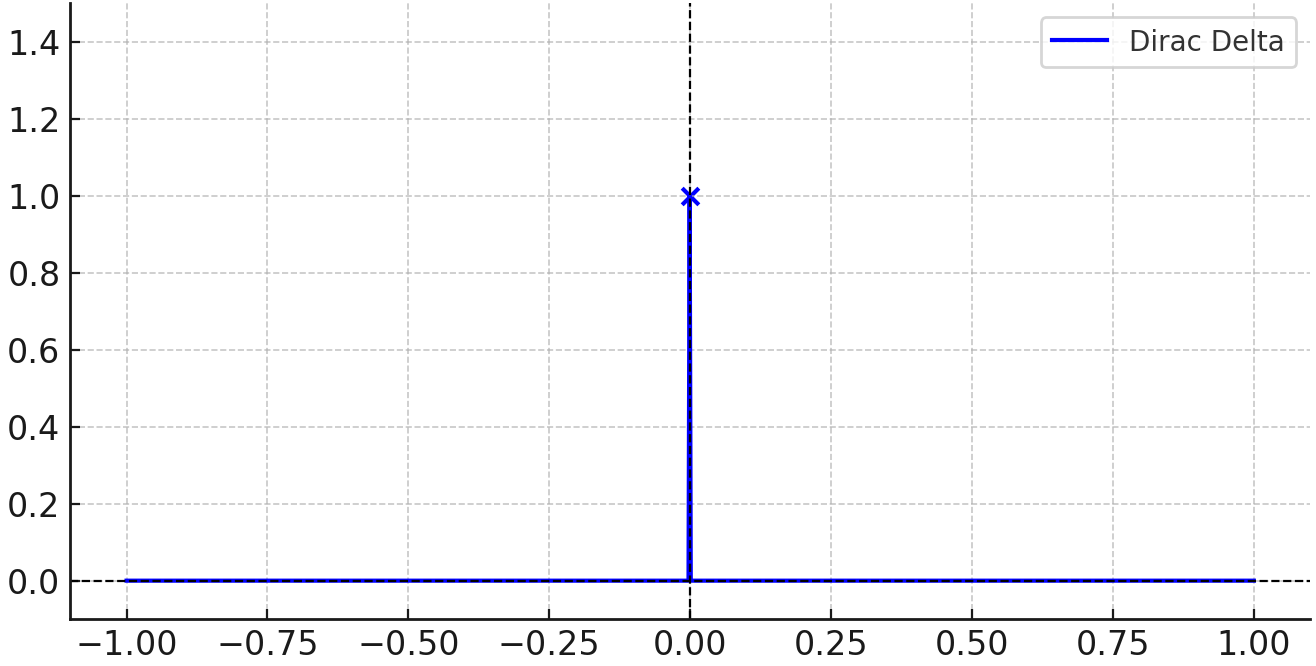
\includegraphics[width=1.1\textwidth]{images/dirac_delta.png}
    \end{center}
\end{minipage}\\

\end{definition}

\noindent
\textbf{Interpretation:} While $\delta_0$ is not a genuine function in the usual sense, it is a linear functional. Every test function $\psi$ is continuous and has compact support, so evaluating $\psi(0)$ is well-defined.

\medskip
\noindent
\textbf{Continuity of $\delta_0$:} We have
\[
|\delta_0(\psi)| = |\psi(0)| \leq \max_{x \in \mathbb{R}}|\psi(x)| \leq C\, \sum_{i=0}^0 \max_{x \in \mathbb{R}}|\psi^{(i)}(x)|,
\]
where we can choose $C = 1$ and $k = 0$. This satisfies the continuity condition in distribution theory.

\medskip
\noindent
\textbf{Symbolic Notation:} Often, one writes
\[
\int_{\mathbb{R}} \delta_0(x)\,\psi(x)\,dx = \psi(0),
\]
emphasizing the \textquoteleft sampling\textquoteright\ property of the delta at $x=0$.

\begin{definition}[Dirac Comb]
The \emph{Dirac comb}, denoted $\Delta_1$, is defined by
\[
\Delta_{1}(\varphi) := \sum_{n \in \mathbb{Z}} \varphi(n),
\]
for each test function $\varphi \in \mathcal{D}$.
\end{definition}

\noindent
\textbf{Properties:}
\begin{itemize}
    \item[-] \emph{Finiteness:} For $\operatorname{supp}(\varphi) \subset [a,b]$, there are finitely many integers in $[a,b]$. Hence
    \[
    \Delta_{1}(\varphi) = \sum_{n \in [a,b] \cap \mathbb{Z}} \varphi(n)
    \]
    is a finite sum.

    \item[-] \emph{Linearity:}
    \[
    \Delta_{1}(\alpha \varphi + \beta \psi)
    = \sum_{n \in \mathbb{Z}} \bigl[\alpha\,\varphi(n) + \beta\,\psi(n)\bigr]
    = \alpha \Delta_{1}(\varphi) + \beta \Delta_{1}(\psi).
    \]

    \item[-] \emph{Continuity:}
    For $\varphi$ with support in $[a,b]$, let $M$ be the number of integers in $[a,b]$. Then
    \[
    |\Delta_{1}(\varphi)|
    \le \sum_{n \in [a,b] \cap \mathbb{Z}} |\varphi(n)|
    \le M \,\max_{x \in \mathbb{R}}|\varphi(x)|.
    \]
    This verifies the required continuity condition in the sense of distributions.
\end{itemize}

\noindent
\textbf{Interpretation:}
$\Delta_1$ can be viewed as a train of impulses (point masses) at every integer point, frequently used in signal processing to represent a periodic sampling process.

\begin{example}[An Integral over \texorpdfstring{$[0,\infty)$}{[0,\infty)}]
\noindent
Consider the distribution $T$ given by
\[
\dist{T}{\varphi} := \int_{0}^{\infty} \varphi(x)\,dx.
\]
\textbf{Properties:}
\begin{itemize}
    \item[-] \emph{Finiteness:}
    If $\mathrm{supp}(\varphi) \subset [a,b]$, then
    \[
    \left|\dist{T}{\varphi}\right|
    = \left| \int_{0}^{\infty} \varphi(x)\,dx \right|
    \le \int_{a}^{b} |\varphi(x)|\,dx
    \le (b-a)\,\max_{x \in \mathbb{R}}|\varphi(x)|.
    \]
    \item[-] \emph{Continuity:}
    For any compact interval $[a,b]$, we can choose $C = (b-a)$ and $k = 0$ to show
    \[
    |\dist{T}{\varphi}| \le C \,\max_{x \in \mathbb{R}}|\varphi(x)|.
    \]
    \item[-] \emph{Linearity:}
    For $\alpha,\beta \in \mathbb{R}$,
    \[
    \dist{T}{\alpha \varphi + \beta \psi}
    = \int_{0}^{\infty} [\alpha\,\varphi(x) + \beta\,\psi(x)]\,dx
    = \alpha \dist{T}{\varphi} + \beta \dist{T}{\psi}.
    \]
\end{itemize}
\end{example}
\begin{example}[Evaluation of a Second Derivative at \texorpdfstring{$\pi$}{pi}]
\noindent
Consider
\[
\dist{T}{\varphi} := \varphi''(\pi).
\]
\textbf{Properties:}
\begin{itemize}
    \item[-] \emph{Finiteness and Continuity:}
    \[
    |\dist{T}{\varphi}| = |\varphi''(\pi)| \le \max_{x \in \mathbb{R}}|\varphi''(x)|,
    \]
    which fits the continuity requirement for distributions.
    \item[-] \emph{Linearity:}
    Follows immediately from the linearity of the second derivative operator:
    \[
    \dist{T}{\alpha \varphi + \beta \psi}
    = (\alpha \varphi + \beta \psi)''(\pi)
    = \alpha\,\varphi''(\pi) + \beta\,\psi''(\pi).
    \]
\end{itemize}
\end{example}
\begin{example}[Shifted Dirac Delta \texorpdfstring{$\delta_a$}{delta\_a}]
\noindent
\textbf{Definition:}
For any $a \in \mathbb{R}$,
\[
\delta_a(\varphi) := \varphi(a).
\]
This is a shift of the delta distribution at 0. In symbolic form, one often writes
\[
\delta_a(x) := \delta(x - a).
\]
Hence $\delta_0$ is a special case with $a=0$.
\end{example}
\begin{example}[Scaled Dirac Comb \texorpdfstring{$\Delta_L$}{Delta\_L}]
\noindent
\textbf{Definition:}
For a positive period $L>0$, the \emph{scaled Dirac comb} is given by
\[
\Delta_L(\varphi) := \sum_{n \in \mathbb{Z}} \varphi(nL),
\]
which can be interpreted as a periodic sequence of impulses at intervals of length $L$.
\end{example}
\bigskip
\section{Derivatives of Distributions}

\subsection{Definition and Motivation}

Let $f \in C^\infty(\mathbb{R})$ be a smooth function and $\varphi \in \mathcal{D}$ be a test function whose support is contained in $[a,b]$. Then
\[
\int_{-\infty}^{\infty} f'(x)\,\varphi(x)\,dx
= \int_{a}^{b} f'(x)\,\varphi(x)\,dx.
\]
Using integration by parts,
\[
\int_{a}^{b} f'(x)\,\varphi(x)\,dx
= \left[ f(x)\,\varphi(x) \right]_{a}^{b} - \int_{a}^{b} f(x)\,\varphi'(x)\,dx.
\]
Since $\varphi$ vanishes at $a$ and $b$ (due to compact support),
\[
\int_{-\infty}^{\infty} f'(x)\,\varphi(x)\,dx
= -\int_{-\infty}^{\infty} f(x)\,\varphi'(x)\,dx.
\]
\begin{definition}[Distributional Derivative]
For a general distribution $f \in \mathcal{D}'$, its \textbf{distributional derivative} $f'$ is defined by
\[
\dist{f'}{\varphi} := -\dist{f}{\varphi'},
\]
for all $\varphi \in \mathcal{D}$.
\end{definition}

\noindent
\textbf{Interpretation:}
This extends the classical idea of differentiation by effectively \emph{transferring} the derivative onto the test function via an integration-by-parts formula.

\subsection{Examples of Distributional Derivatives}

\begin{example}[A $C^1$ Function]
If $f \in C^1(\mathbb{R})$, then in the distribution sense,
\[
f'_\text{distributional} = f'_\text{classical}.
\]
Hence the distributional derivative agrees with the usual one for sufficiently smooth functions.
\end{example}

\begin{example}[Derivative of an Integral Functional]
Define
\[
\dist{T}{\varphi} := \int_{-\infty}^{\infty} \varphi(x)\,dx.
\]
Then, using the definition of the distributional derivative,
\[
\dist{T'}{\varphi}
= -\dist{T}{\varphi'}
= -\int_{-\infty}^{\infty} \varphi'(x)\,dx
= \varphi(0),
\]
by the fundamental theorem of calculus. This equals $\delta_0(\varphi)$, so
\[
T' = \delta_0.
\]
Alternatively, we can view $T$ as coming from the \emph{Heaviside function}
\[
H(x) =
\begin{cases}
0, & x < 0, \\
1, & x \ge 0,
\end{cases}
\]
whose derivative (in the distribution sense) is $\delta_0$.
\end{example}

\begin{example}[Jump Distributions]
Let
\[
\dist{T}{\varphi} := \int_0^1 \varphi(x)\,dx.
\]
Then
\[
\dist{T'}{\varphi} = -\int_0^1 \varphi'(x)\,dx
= -\varphi(1) + \varphi(0),
\]
which can be written as
\[
\dist{T'}{\varphi} = -\,\delta_1(\varphi) + \delta_0(\varphi).
\]
Equivalently, this distribution arises from the characteristic function of $[0,1]$:
\[
g(x) =
\begin{cases}
1, & 0 \le x \le 1, \\
0, & \text{otherwise}.
\end{cases}
\]
Its distributional derivative captures the jumps at $0$ and $1$.
\end{example}

\subsection{Distributional Derivatives of Piecewise Differentiable Functions}

\noindent
Suppose $f: \mathbb{R} \to \mathbb{R}$ is piecewise continuous and piecewise differentiable, with possible jump discontinuities at points $a_0 < a_1 < \cdots < a_n$. For each test function $\varphi$,
\[
\dist{f'}{\varphi}
= -\dist{f}{\varphi'}
= -\int_{-\infty}^{\infty} f(x)\,\varphi'(x)\,dx.
\]
Breaking the integral into intervals and performing integration by parts on each sub-interval, we see that:
\[
\dist{f'}{\varphi}
= \int_{-\infty}^{a_0} f'(x)\,\varphi(x)\,dx + \sum_{i=1}^{n} \int_{a_{i-1}}^{a_i} f'(x)\,\varphi(x)\,dx + \int_{a_n}^{\infty} f'(x)\,\varphi(x)\,dx
+ \sum_{i=0}^{n} \varphi(a_i)\,\bigl[f(a_i^-) - f(a_i^+)\bigr].
\]
Hence, the distributional derivative consists of:
\begin{itemize}
    \item[-] The classical derivative $f'(x)$ in each smooth region.
    \item[-] Additional \emph{Dirac delta} terms at each jump discontinuity $a_i$, weighted by the jump $f(a_i^-)-f(a_i^+)$.
\end{itemize}

\subsection{Specific Examples}

\begin{example}[Hat Function]
Consider the \textbf{hat function}:
\[
f(x) =
\begin{cases}
0, & x < -1,\\
x + 1, & -1 \le x < 0,\\
1 - x, & 0 \le x < 1,\\
0, & x \ge 1.
\end{cases}
\]
Since $f$ is continuous and piecewise linear,
\[
f'(x) =
\begin{cases}
0, & x < -1,\\
1, & -1 < x < 0,\\
-1, & 0 < x < 1,\\
0, & x > 1.
\end{cases}
\]
This is also the \emph{weak derivative}. The \emph{second} distributional derivative involves the jumps in $f'(x)$:
\[
f''(x) = \delta_{-1} - 2\,\delta_{0} + \delta_{1}.
\]
\end{example}

\begin{example}[Heaviside Function]
The \textbf{Heaviside function} $H(x)$,
\[
H(x) =
\begin{cases}
0, & x < 0,\\
1, & x \ge 0,
\end{cases}
\]
has the distributional derivative
\[
H'(x) = \delta_0.
\]
\end{example}

\begin{example}[Staircase Function]
Consider a \textbf{staircase function} with integer steps,
\[
f(x) = n, \quad \text{if } x \in [n-1,n), \; n \in \mathbb{Z}.
\]
Its distributional derivative is
\[
f'(x) = \sum_{n \in \mathbb{Z}} \delta_n,
\]
often called a \emph{Dirac comb}.
\end{example}

\subsection{Derivatives of the Dirac Delta}

\noindent
For the Dirac delta $\delta_0$, higher-order derivatives are defined by
\[
\dist{\delta_0^{(n)}}{\varphi}
= (-1)^n \,\varphi^{(n)}(0).
\]
This highlights the principle that differentiating a delta distribution results in a new distribution that \textquoteleft samples\textquoteright\ higher-order derivatives of the test function at the origin.

\medskip
\begin{center}
  \hrulefill
\end{center}

\end{document}
